\documentclass[a4paper,11pt]{report}
\usepackage[showexo=true,showcorr=false]{../packages/coursclasse}
%Commenter ou enlever le commentaire sur la ligne suivante pour montrer le niveau
\toggletrue{montrerNiveaux}
%permet de gérer l'espacement entre les items des env enumerate et enumitem
\usepackage{enumitem}
\setlist[enumerate]{align=left,leftmargin=1cm,itemsep=10pt,parsep=0pt,topsep=0pt,rightmargin=0.5cm}
\setlist[itemize]{align=left,labelsep=1em,leftmargin=*,itemsep=0pt,parsep=0pt,topsep=0pt,rightmargin=0cm}
%permet de gerer l'espacement entre les colonnes de multicols
\setlength\columnsep{20pt}

\begin{document}

%%%%%%%%%%%%%%%%% À MODIFIER POUR CHAQUE SERIE %%%%%%%%%%%%%%%%%%%%%%%%%%%%%
\newcommand{\chapterName}{Espace}
\newcommand{\serieName}{Classification des quadrilatères}


%%%%%%%%%%%%%%%%%% PREMIERE PAGE NE PAS MODIFER %%%%%%%%%%%%%%%%%%%%%%%%
% le chapitre en cours, ne pas changer au cours d'une série
\chapter*{\chapterName}
\thispagestyle{empty}

%%%%% LISTE AIDE MEMOIRE %%%%%%
\begin{amL}{\serieName}{
\item Quadrilatère (page 123)
\item Quadrilatères particuliers (pages 123-124)
\item Classement des quadrilatères (page 125)
\item Diagonale d'un polygone (page 111)
}\end{amL}

%%%%%%%%%%%%%%% DEBUT DE LA SERIE NE PAS MODIFIER %%%%%%%%%%%%%%%%%%%%%%%%%%%%%
\section*{\serieName}
\setcounter{page}{1}
\thispagestyle{firstPage}





%%%%%%%%%%% LES EXERCICES %%%%%%%%%%%%%%%%%%%%%%%%%%%%%%%%%%%%

\begin{exop}{
		\begin{minipage}[t]{0.4\textwidth}{
		\vspace{0pt}
		   Complète les phrases en utilisant les mots "côtés", "sommets" ou "diagonales" et "opposés" ou "consécutifs".
		}
		\end{minipage}
		\hfill
		\begin{minipage}[t]{0.4\textwidth}{
		\vspace{0pt}
   \begin{center}
	    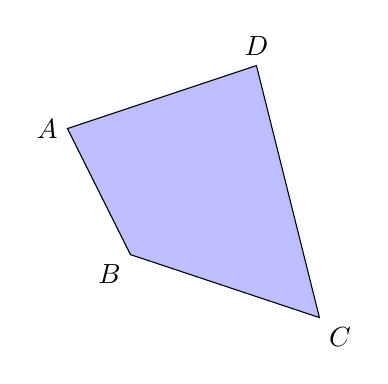
\begin{tikzpicture}[scale=0.8]
            \draw[fill=blue!25] (0,0) -- (1,-2) -- (4,-3) -- (3,1) -- cycle ;
            \node[left] at (0,0) {$A$} ; 
            \node[below left] at (1,-2) {$B$} ;
            \node[below right] at (4,-3) {$C$} ;
            \node[above] at (3,1) {$D$} ;
        \end{tikzpicture}
    \end{center}
		}
		\end{minipage}
    \begin{tasks}(1)
        \task $AB$ et $CD$ sont des ~\hrulefill \quad \ligne{5}.
        \task $C$ et $D$ sont des ~\hrulefill \quad \ligne{5}.
        \task $AD$ et $BC$ sont des ~\hrulefill \quad \ligne{5}.
        \task $AC$ et $BD$ sont les ~\hrulefill \quad \ligne{5}.
        \task $A$ et $C$ sont des ~\hrulefill \quad \ligne{5}.
        \task $AB$ et $BC$ sont des ~\hrulefill \quad \ligne{5}.
    \end{tasks}
}{1}
\end{exop}


\begin{exop}{
		\begin{minipage}[t]{0.5\textwidth}{
		\vspace{0pt}
		    Complète les phrases en utilisant les mots "côtés", "sommets" ou "diagonales" et "opposés" ou "consécutifs".
		}
		\end{minipage}
		\hfill
		\begin{minipage}[t]{0.4\textwidth}{
		\vspace{0pt}
 \begin{center}
	    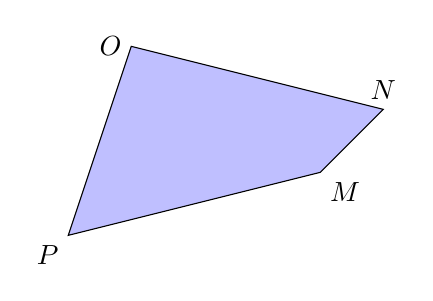
\begin{tikzpicture}[scale=0.8]
            \draw[fill=blue!25] (0,0) -- (-1,-3) -- (3,-2) -- (4,-1) -- cycle ;
            \node[left] at (0,0) {$O$} ; 
            \node[below left] at (-1,-3) {$P$} ;
            \node[below right] at (3,-2) {$M$} ;
            \node[above] at (4,-1) {$N$} ;
        \end{tikzpicture}
    \end{center}
		}
		\end{minipage}

    \begin{tasks}(1)
        \task $OP$ et $PM$ sont des ~\hrulefill \quad \ligne{5}.
        \task $M$ et $N$ sont des ~\hrulefill \quad \ligne{5}.
        \task $OP$ et $MN$ sont des ~\hrulefill \quad \ligne{5}.
        \task $O$ et $M$ sont des ~\hrulefill \quad \ligne{5}.
        \task $ON$ et $PM$ sont des ~\hrulefill \quad \ligne{5}.
        \task $OM$ et $PN$ sont les ~\hrulefill \quad \ligne{5}.
    \end{tasks}
}{1}
\end{exop}

%begin{\exo}{
%    Place les noms des quadrilatères dans le diagramme. \\

%    J'imagine reproduire un diagramme (en une ou plusieurs parties) comme dans l'aide mémoire.
%}{2}


\begin{exo}{
    Pour chaque figure, fais un croquis dans ton cahier, puis coche (\makebox[0pt][l]{$\checkmark$}$\square$) la ou les bonnes réponses. \\
    {\small \textit{(Vocabulaire : un quadrilatère de centre O est un quadrilatère dont les diagonales se croisent en O.)}}
    
    
    \begin{tasks}
        \task ABCD est un rectangle de centre O.  Alors $\ldots$
        {\setlength\columnsep{-10pt}
        \begin{multicols}{4}
        \begin{enumerate}[label=$\square$]
            \item AB=BC
            \item BC=AD
            \item AC=BD
            \item OA=OB
        \end{enumerate}
        \end{multicols}}
        \task GHJK est un losange de centre M. Alors $\ldots$
        {\setlength\columnsep{-10pt}
        \begin{multicols}{4}
        \begin{enumerate}[label=$\square$]
            \item GH=HJ
            \item GJ=HK
            \item MG=MH
            \item MG=MJ
        \end{enumerate}
        \end{multicols}}

        
        \task EFGH est un rectangle. Alors ses diagonales $\ldots$
        {\setlength\columnsep{-10pt}
        \begin{multicols}{2}
        \begin{enumerate}[label=$\square$]
            \item sont perpendiculaires
            \item sont de même longueur
            \item se coupent en leur milieu
            \item sont parallèles
        \end{enumerate}
        \end{multicols}}
        
        \task RSTU est un losange. Alors ses diagonales $\ldots$
       {\setlength\columnsep{-10pt}
        \begin{multicols}{2}
        \begin{enumerate}[label=$\square$]
            \item sont perpendiculaires
            \item sont de même longueur
            \item se coupent en leur milieu
            \item sont parallèles
        \end{enumerate}
        \end{multicols}}
\end{tasks}
}{1}
\end{exo}



\begin{exo}{
    Pour chaque figure, fais un croquis, puis coche (\makebox[0pt][l]{$\checkmark$}$\square$) la ou les bonnes réponses. \\
    {\small \textit{(Vocabulaire : Un quadrilatère de centre O est un quadrilatère dont les diagonales se croisent en O.)}}
    
    
    \begin{tasks}
        
        \task ABCD est un rectangle. Alors ses diagonales $\ldots$
        {\setlength\columnsep{-10pt}
        \begin{multicols}{2}
        \begin{enumerate}[label=$\square$]
            \item sont perpendiculaires
            \item sont de même longueur
            \item se coupent en leur milieu
            \item sont parallèles
        \end{enumerate}
        \end{multicols}}
        
        \task EFGH est un losange de centre L. Alors $\ldots$
        {\setlength\columnsep{-10pt}
        \begin{multicols}{4}
        \begin{enumerate}[label=$\square$]
            \item EF=FG
            \item EG=FH
            \item LE=LF
            \item LE=LG
        \end{enumerate}
        \end{multicols}}
        
        \task IJKL est un losange. Alors ses diagonales $\ldots$
       {\setlength\columnsep{-10pt}
        \begin{multicols}{2}
        \begin{enumerate}[label=$\square$]
            \item sont perpendiculaires
            \item sont de même longueur
            \item se coupent en leur milieu
            \item sont parallèles
        \end{enumerate}
        \end{multicols}}

        \task MNOP est un rectangle de centre Q.  Alors $\ldots$
        {\setlength\columnsep{-10pt}
        \begin{multicols}{4}
        \begin{enumerate}[label=$\square$]
            \item MN=NO
            \item NO=MP
            \item MO=NP
            \item QM=QN
        \end{enumerate}
        \end{multicols}}
\end{tasks}
}{1}
\end{exo}

\begin{QSJ}{131}{1}
\end{QSJ}
\begin{exol}{ES74}{111}{1}
\end{exol}
\begin{exof}{ES75}{133}{1}
\end{exof}
\begin{exol}{ES82}{112}{1}
\end{exol}

						\begin{exo}{
    Donne le nom exact des quadrilatères décrits ci-dessous.

    \begin{tasks}(1)
        \task J'ai toutes les propriétés du losange, et en plus, des angles droits. %1

        \task J'ai deux paires de côtés parallèles, quatre angles droits et deux axes de symétries. %1

        \task Mes deux diagonales sont isométriques et forment un angle droit. %1

        \task J'ai quatre côtés isométriques mais aucun angle droit. %1

        \task Je n'ai qu'une seule paire de côtés parallèles. %1

        \task Je n'ai qu'une seule paire de côtés parallèles et un seul axe de symétrie. %1
    \end{tasks}
}{1}
\end{exo}

\begin{exo}{
    Donne le nom exact des quadrilatères décrits ci-dessous.

    \begin{tasks}(1)        
        \task J'ai une paire de côtés parallèles et deux angles droits. %2

        \task J'ai un axe de symétrie et je suis le seul à ne pas être convexe. %2
        
        \task J'ai deux paires de côtés isométriques et je n'ai pas d'axe de symétrie. %2

        \task J'ai deux paires de côtés parallèles et isométriques, mais je n'ai pas d'axe de symétrie. %2

        \task C'est moi qui possède le plus d'axes de symétrie. %2

        \task Je n'ai que deux axes de symétries et ils se confondent avec mes diagonales. %2
    \end{tasks}
}{2}
\end{exo}


\begin{exo}{
    $PQRS$ est un losange de centre $O$. Détermine les mesures demandées en justifiant par une propriété du losange. \\
    \begin{center}
    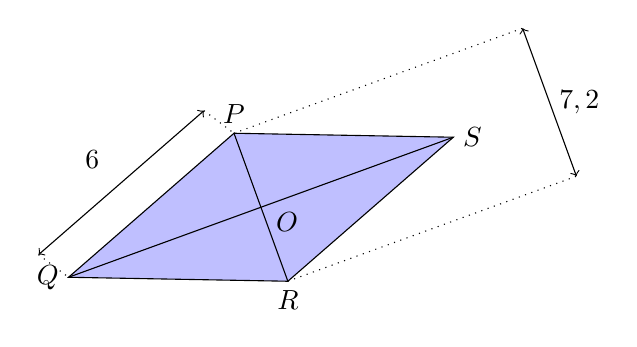
\begin{tikzpicture}[rotate=20, xscale=1.3]
        \draw[fill=blue!25] (-2,0) -- (0,-1) -- (2,0) -- (0,1) -- cycle ;
        \draw[<->] (-2.2,0.4) -- (-0.2,1.4) ;
        \draw[dotted] (-2.2,0.4) -- (-2,0) ;
        \draw[dotted] (-0.2,1.4) -- (0,1) ;
	\node[above left] at (-1.3,1) {$\tunit{6}{\cm}$} ;
        \draw[] (-2,0) -- (2,0) ;
        \draw[] (0,1) -- (0,-1) ;
        \draw[dotted] (0,1)--(3,1);
        \draw[dotted] (0,-1)--(3,-1);
        \draw[<->] (3,-1)--(3,1) ;
	\node[right] at (3,0) {$\tunit{7,2}{\cm}$} ;
        \node[above] at (0,1) {$P$} ;
        \node[right] at (2,0) {$S$} ;
        \node[below] at (0,-1) {$R$} ;
        \node[left] at (-2,0) {$Q$} ;
        \node[above, right] at (0,-0.2) {$O$} ;
    \end{tikzpicture}
    \end{center}
    
    \begin{tasks}(3)
        \task la longueur $SR$ ;
        \task la longueur $PO$ ;
        \task l'angle $\widehat{SOP}$.
    \end{tasks}
}{1}
\end{exo}

\begin{exo}{
    $JKLM$ est un losange de centre $O$. Détermine les mesures demandées en justifiant par une propriété du losange. \\
    \begin{center}
    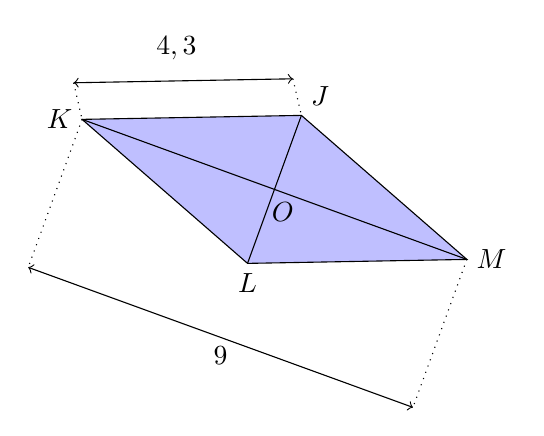
\begin{tikzpicture}[rotate=-20, xscale=1.3]
        \draw[fill=blue!25] (-2,0) -- (0,-1) -- (2,0) -- (0,1) -- cycle ;
        \draw[<->] (-2.2,0.4) -- (-0.2,1.4) ;
        \draw[dotted] (-2.2,0.4) -- (-2,0) ;
        \draw[dotted] (-0.2,1.4) -- (0,1) ;
	\node[above] at (-1.3,1) {$\tunit{4,3}{\cm}$} ;
        \draw[] (-2,0) -- (2,0) ;
        \draw[] (0,1) -- (0,-1) ;
        \draw[dotted] (-2,0)--(-2,-2);
        \draw[dotted] (2,0)--(2,-2);
        \draw[<->] (-2,-2)--node[below, sloped]{$\tunit{9}{\cm}$}(2,-2) ;
	%\node[right] at (3,0) {$\tunit{7,2}{\cm}$} ;
        \node[above right] at (0,1) {$J$} ;
        \node[right] at (2,0) {$M$} ;
        \node[below] at (0,-1) {$L$} ;
        \node[left] at (-2,0) {$K$} ;
        \node[below right] at (-0.1,-0.1) {$O$} ;
    \end{tikzpicture}
    \end{center}
    
    \begin{tasks}(3)
        \task la longueur $KL$ 
        \task la longueur $OM$ 
        \task l'angle $\widehat{JOK}$
    \end{tasks}
}{1}
\end{exo}

\newpage
\begin{exo}{
    $ABCD$ est le rectangle ci-contre. Quelles sont les longueurs des segments $CD$ et $BD$~? Justifie en citant les propriétés d'un rectangle.
    \begin{center}
        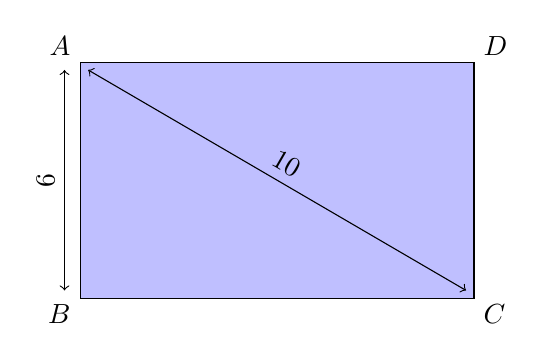
\begin{tikzpicture}
            \draw[fill=blue!25] (0,0) -- (5,0) -- (5,3) -- (0,3) -- cycle ;
            \draw[<->] (0.1,2.9) -- (4.9,0.1) ;
	    \node[above, rotate=-30] at (2.5,1.5) {$\tunit{10}{\cm}$} ;
            \draw[<->] (-0.2,0.1) -- (-0.2,2.9) ;
	    \node[above, rotate=90] at (-0.2,1.5) {$\tunit{6}{\cm}$} ;
            \node[above, left] at (0,3.2) {$A$} ;
            \node[below, left] at (0,-0.2) {$B$} ;
            \node[below, right] at (5,-0.2) {$C$} ;
            \node[above, right] at (5,3.2) {$D$} ;
            
        \end{tikzpicture}
    \end{center}
}{1}
\end{exo}


\begin{exo}{
    $RSTU$ est le rectangle ci-contre. Quelles sont les longueurs des segments $TS$ et $TR$~? Justifie en citant les propriétés d'un rectangle.
    \begin{center}
        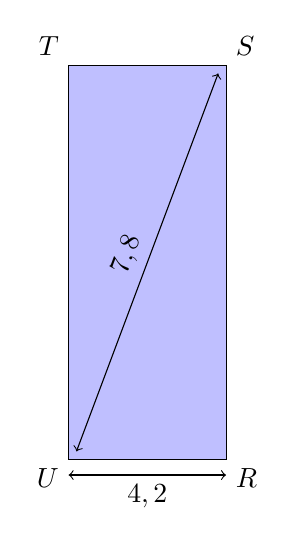
\begin{tikzpicture}
            \draw[fill=blue!25] (0,0) -- (2,0) -- (2,5) -- (0,5) -- cycle ;
            \draw[<->] (0.1,0.1) --node[above, sloped]{$\tunit{7,8}{\cm}$} (1.9,4.9) ;
	    %\node[above, rotate=-30] at (2.5,1.5) {$\tunit{10}{\cm}$} ;
            \draw[<->] (0,-0.2) --node[below,sloped] {$\tunit{4,2}{\cm}$} (2,-0.2) ;
	    %\node[above, rotate=90] at (-0.2,1.5) {$\tunit{6}{\cm}$} ;
            \node[above left] at (0,5) {$T$} ;
            \node[below left] at (0,0) {$U$} ;
            \node[below right] at (2,0) {$R$} ;
            \node[above right] at (2,5) {$S$} ;
            
        \end{tikzpicture}
    \end{center}
}{1}
\end{exo}

\newpage

\begin{exop}{
\begin{tasks}
    \task S'ils existent, trace les axes de symétries des quadrilatères suivants. Sois précis, utilise tes instruments de géométrie.
	    \vspace{-0.3cm}
    \begin{center}
        \begin{center}
    \begin{tikzpicture}

    \begin{scope}[xshift=-1cm, yshift=2cm, rotate=90, scale=0.4]
        %\begin{tikzpicture}
    \draw (0,0) -- (5,0) -- (3,3) -- (0,3) -- cycle ;
%\end{tikzpicture}
    \end{scope}
    
    \begin{scope}[rotate=-5, scale=0.6]
        %\begin{tikzpicture}
    \draw (0,0) -- (0,2) -- (2,2) -- (2,0) -- cycle ;
%\end{tikzpicture}
    \end{scope}

    \begin{scope}[xshift=3cm, yshift=3cm, rotate=30, scale=0.5]
        %\begin{tikzpicture}
    \draw (0,0) -- (2,-5) -- (4,0) -- (2,-2) -- cycle ;
%\end{tikzpicture}
    \end{scope}
    
    \begin{scope}[xshift=3.5cm, yshift=-2cm, rotate=40, scale=0.4]
        %\begin{tikzpicture}
    \draw (0,0) -- (2,-5) -- (4,0) -- (2,5) -- cycle ;
%\end{tikzpicture}
    \end{scope}

    \begin{scope}[xshift=10cm, yshift=-4cm, rotate=45,  scale=0.6]
        %\begin{tikzpicture}
    \draw (0,0) -- (5,0) -- (3,3) -- (2,3) -- cycle ;
%\end{tikzpicture}
    \end{scope}

    \begin{scope}[xshift=9cm, yshift=1cm, rotate=15, scale=0.6]
        %\begin{tikzpicture}
    \draw (0,0) -- (5,0) -- (3,2) -- (-2,2) -- cycle ;
%\end{tikzpicture}
    \end{scope}

    \begin{scope}[yshift=-4cm, xshift=-1cm, rotate=75, scale=0.4]
        %\begin{tikzpicture}
    \draw (0,0) -- (2,-5) -- (4,0) -- (2,3) -- cycle ;
%\end{tikzpicture}
    \end{scope}
    
    \begin{scope}[yshift=-8cm, xshift=-2cm, rotate=-15, scale=0.6]
        %\begin{tikzpicture}
    \draw (0,0) -- (7,0) -- (3,3) -- (2,3) -- cycle ;
%\end{tikzpicture}
    \end{scope}

    \begin{scope}[yshift=-7cm, xshift=4cm, rotate=10, scale=0.7]
        %\begin{tikzpicture}
    \draw (0,0) -- (0,2) -- (5,2) -- (5,0) -- cycle ;
%\end{tikzpicture}
    \end{scope}

    \begin{scope}[yshift=-9.5cm, xshift=7cm, rotate=10, scale=0.6]
        %\begin{tikzpicture}
    \draw (0,0) -- (5,0) -- (10,2) -- (5,2) -- cycle ;
%\end{tikzpicture}
    \end{scope}
    
    \end{tikzpicture}
    \end{center}

    \end{center}
    
    \task Nomme les figures qui possèdent au moins un axe de symétrie. 

	    \ligne{14}

    \task Nomme les figures qui possèdent deux axes de symétrie.  

	    \ligne{14}

    \task Nomme les figures qui ne possèdent aucun axe de symétrie. 

	    \ligne{14}
\end{tasks}
    
}{1}
\end{exop}



\begin{exop}{
\begin{tasks}
    \task S'il y en a, trace en couleur les paires de côtés parallèles des quadrilatères suivants.
\vspace{-0.2cm}
    \begin{center}
    \begin{center}
    \begin{tikzpicture}

    \begin{scope}[xshift=-1cm, yshift=2cm, rotate=90, scale=0.4]
        %\begin{tikzpicture}
    \draw (0,0) -- (5,0) -- (3,3) -- (0,3) -- cycle ;
%\end{tikzpicture}
    \end{scope}
    
    \begin{scope}[rotate=-5, scale=0.6]
        %\begin{tikzpicture}
    \draw (0,0) -- (0,2) -- (2,2) -- (2,0) -- cycle ;
%\end{tikzpicture}
    \end{scope}

    \begin{scope}[xshift=3cm, yshift=3cm, rotate=30, scale=0.5]
        %\begin{tikzpicture}
    \draw (0,0) -- (2,-5) -- (4,0) -- (2,-2) -- cycle ;
%\end{tikzpicture}
    \end{scope}
    
    \begin{scope}[xshift=3.5cm, yshift=-2cm, rotate=40, scale=0.4]
        %\begin{tikzpicture}
    \draw (0,0) -- (2,-5) -- (4,0) -- (2,5) -- cycle ;
%\end{tikzpicture}
    \end{scope}

    \begin{scope}[xshift=10cm, yshift=-4cm, rotate=45,  scale=0.6]
        %\begin{tikzpicture}
    \draw (0,0) -- (5,0) -- (3,3) -- (2,3) -- cycle ;
%\end{tikzpicture}
    \end{scope}

    \begin{scope}[xshift=9cm, yshift=1cm, rotate=15, scale=0.6]
        %\begin{tikzpicture}
    \draw (0,0) -- (5,0) -- (3,2) -- (-2,2) -- cycle ;
%\end{tikzpicture}
    \end{scope}

    \begin{scope}[yshift=-4cm, xshift=-1cm, rotate=75, scale=0.4]
        %\begin{tikzpicture}
    \draw (0,0) -- (2,-5) -- (4,0) -- (2,3) -- cycle ;
%\end{tikzpicture}
    \end{scope}
    
    \begin{scope}[yshift=-8cm, xshift=-2cm, rotate=-15, scale=0.6]
        %\begin{tikzpicture}
    \draw (0,0) -- (7,0) -- (3,3) -- (2,3) -- cycle ;
%\end{tikzpicture}
    \end{scope}

    \begin{scope}[yshift=-7cm, xshift=4cm, rotate=10, scale=0.7]
        %\begin{tikzpicture}
    \draw (0,0) -- (0,2) -- (5,2) -- (5,0) -- cycle ;
%\end{tikzpicture}
    \end{scope}

    \begin{scope}[yshift=-9.5cm, xshift=7cm, rotate=10, scale=0.6]
        %\begin{tikzpicture}
    \draw (0,0) -- (5,0) -- (10,2) -- (5,2) -- cycle ;
%\end{tikzpicture}
    \end{scope}
    
    \end{tikzpicture}
    \end{center}

    \end{center}
    
    \task Nomme les figures qui ont au moins une paire de côtés parallèles.  

	    \ligne{14}

    \task Nomme les figures qui ont deux paires de côtés parallèles.

	     \ligne{14}

    \task Nomme les figures qui n'ont aucune paire de côtés parallèles.  

	    \ligne{14}
\end{tasks}
    
}{1}
\end{exop}

\begin{exop}{
\begin{tasks}
    \task S'il y en a, trace en couleur les côtés isométriques des quadrilatères suivants. 
	    \vspace{-0.3cm}
    \begin{center}
    \begin{center}
    \begin{tikzpicture}

    \begin{scope}[xshift=-1cm, yshift=0cm, rotate=90, scale=0.4]
        %\begin{tikzpicture}
    \draw (0,0) -- (5,0) -- (3,3) -- (0,3) -- cycle ;
%\end{tikzpicture}
    \end{scope}
    
    \begin{scope}[yshift=-1cm, rotate=-5, scale=0.6]
        %\begin{tikzpicture}
    \draw (0,0) -- (0,2) -- (2,2) -- (2,0) -- cycle ;
%\end{tikzpicture}
    \end{scope}

    \begin{scope}[xshift=3cm, yshift=1.5cm, rotate=30, scale=0.5]
        %\begin{tikzpicture}
    \draw (0,0) -- (2,-5) -- (4,0) -- (2,-2) -- cycle ;
%\end{tikzpicture}
    \end{scope}
    
    \begin{scope}[xshift=3.5cm, yshift=-2cm, rotate=40, scale=0.4]
        %\begin{tikzpicture}
    \draw (0,0) -- (2,-5) -- (4,0) -- (2,5) -- cycle ;
%\end{tikzpicture}
    \end{scope}

    \begin{scope}[xshift=10cm, yshift=-4cm, rotate=45,  scale=0.6]
        %\begin{tikzpicture}
    \draw (0,0) -- (5,0) -- (3,3) -- (2,3) -- cycle ;
%\end{tikzpicture}
    \end{scope}

    \begin{scope}[xshift=9cm, yshift=0cm, rotate=15, scale=0.6]
        %\begin{tikzpicture}
    \draw (0,0) -- (5,0) -- (3,2) -- (-2,2) -- cycle ;
%\end{tikzpicture}
    \end{scope}

    \begin{scope}[yshift=-4cm, xshift=-1cm, rotate=75, scale=0.4]
        %\begin{tikzpicture}
    \draw (0,0) -- (2,-5) -- (4,0) -- (2,3) -- cycle ;
%\end{tikzpicture}
    \end{scope}
    
    \begin{scope}[yshift=-7cm, xshift=-2cm, rotate=-15, scale=0.6]
        %\begin{tikzpicture}
    \draw (0,0) -- (7,0) -- (3,3) -- (2,3) -- cycle ;
%\end{tikzpicture}
    \end{scope}

    \begin{scope}[yshift=-6cm, xshift=4cm, rotate=10, scale=0.7]
        %\begin{tikzpicture}
    \draw (0,0) -- (0,2) -- (5,2) -- (5,0) -- cycle ;
%\end{tikzpicture}
    \end{scope}

    \begin{scope}[yshift=-8cm, xshift=7cm, rotate=10, scale=0.6]
        %\begin{tikzpicture}
    \draw (0,0) -- (5,0) -- (10,2) -- (5,2) -- cycle ;
%\end{tikzpicture}
    \end{scope}
    
    \end{tikzpicture}
    \end{center}

    \end{center}
    \vspace{-0.6cm}
    
    \task Nomme les figures qui possèdent une paire de côtés isométriques. 

	    \ligne{14}

    \task Nomme les figures qui possèdent deux paires de côtés isométriques. 

	    \ligne{14}

    \task Nomme les figures qui possèdent quatre côtés isométriques. 

	    \ligne{14}
    
    \task Nomme les figures qui ne possèdent aucune paire de côtés isométriques. 

	    \ligne{14}

\end{tasks}
    
}{1}
\end{exop}

\begin{exop}{
\begin{tasks}
    \task Trace les diagonales des quadrilatères suivants.
	    \vspace{-0.2cm}
    \begin{center}
    \begin{center}
    \begin{tikzpicture}

    \begin{scope}[xshift=-1cm, yshift=2cm, rotate=90, scale=0.4]
        %\begin{tikzpicture}
    \draw (0,0) -- (5,0) -- (3,3) -- (0,3) -- cycle ;
%\end{tikzpicture}
    \end{scope}
    
    \begin{scope}[rotate=-5, scale=0.6]
        %\begin{tikzpicture}
    \draw (0,0) -- (0,2) -- (2,2) -- (2,0) -- cycle ;
%\end{tikzpicture}
    \end{scope}

    \begin{scope}[xshift=3cm, yshift=3cm, rotate=30, scale=0.5]
        %\begin{tikzpicture}
    \draw (0,0) -- (2,-5) -- (4,0) -- (2,-2) -- cycle ;
%\end{tikzpicture}
    \end{scope}
    
    \begin{scope}[xshift=3.5cm, yshift=-2cm, rotate=40, scale=0.4]
        %\begin{tikzpicture}
    \draw (0,0) -- (2,-5) -- (4,0) -- (2,5) -- cycle ;
%\end{tikzpicture}
    \end{scope}

    \begin{scope}[xshift=10cm, yshift=-4cm, rotate=45,  scale=0.6]
        %\begin{tikzpicture}
    \draw (0,0) -- (5,0) -- (3,3) -- (2,3) -- cycle ;
%\end{tikzpicture}
    \end{scope}

    \begin{scope}[xshift=9cm, yshift=1cm, rotate=15, scale=0.6]
        %\begin{tikzpicture}
    \draw (0,0) -- (5,0) -- (3,2) -- (-2,2) -- cycle ;
%\end{tikzpicture}
    \end{scope}

    \begin{scope}[yshift=-4cm, xshift=-1cm, rotate=75, scale=0.4]
        %\begin{tikzpicture}
    \draw (0,0) -- (2,-5) -- (4,0) -- (2,3) -- cycle ;
%\end{tikzpicture}
    \end{scope}
    
    \begin{scope}[yshift=-8cm, xshift=-2cm, rotate=-15, scale=0.6]
        %\begin{tikzpicture}
    \draw (0,0) -- (7,0) -- (3,3) -- (2,3) -- cycle ;
%\end{tikzpicture}
    \end{scope}

    \begin{scope}[yshift=-7cm, xshift=4cm, rotate=10, scale=0.7]
        %\begin{tikzpicture}
    \draw (0,0) -- (0,2) -- (5,2) -- (5,0) -- cycle ;
%\end{tikzpicture}
    \end{scope}

    \begin{scope}[yshift=-9.5cm, xshift=7cm, rotate=10, scale=0.6]
        %\begin{tikzpicture}
    \draw (0,0) -- (5,0) -- (10,2) -- (5,2) -- cycle ;
%\end{tikzpicture}
    \end{scope}
    
    \end{tikzpicture}
    \end{center}

    \end{center}
    
    \task Nomme les figures dont les diagonales se coupent en leur milieu. \ligne{14}

    \task Nomme les figures dont les diagonales se coupent à angle droit. 

	    \ligne{14}

\end{tasks}
    
}{1}
\end{exop}



\newpage

\begin{exop}{ 
Complète le tableau avec tes observations obtenues aux exercices précédent. \\


\begin{tabular}{|*{5}{p{2.8cm}|}}
\hline
Quadrilatère & Axe(s) de symétrie & Côtés isométriques & Diagonales & Nom du quadrilatère \\ \hline

\begin{tikzpicture}
    \clip (-2,-0.5) rectangle (2,2.5) ;
    \begin{scope}[rotate=90, scale=0.4]
        %\clip (-0.5,-0.5) rectangle (5.5,4.5) ;
        %\begin{tikzpicture}
    \draw (0,0) -- (5,0) -- (3,3) -- (0,3) -- cycle ;
%\end{tikzpicture}
    \end{scope}
\end{tikzpicture}
&&&& \\ \hline

\begin{tikzpicture}
    \clip (-0.5,-1) rectangle (3.5,2) ;
    \begin{scope}[rotate=-5, scale=0.6]
        %\clip (-1,-0.5) rectangle (2.5,2.5) ;
        %\begin{tikzpicture}
    \draw (0,0) -- (0,2) -- (2,2) -- (2,0) -- cycle ;
%\end{tikzpicture}
    \end{scope}
\end{tikzpicture} &&&& \\ \hline

\begin{tikzpicture}
    \clip (-0.5,-2) rectangle (3.5,2) ;
    \begin{scope}[rotate=30, scale=0.4]
        %\clip (-0.5,-5.1) rectangle (4.1,0.5) ;
        %\begin{tikzpicture}
    \draw (0,0) -- (2,-5) -- (4,0) -- (2,-2) -- cycle ;
%\end{tikzpicture}
    \end{scope}
\end{tikzpicture} &&&& \\ \hline

\begin{tikzpicture}
    \clip (-1,-1) rectangle (3,2) ;
    \begin{scope}[rotate=40, scale=0.3]
        %\clip (-0.1,-5.1) rectangle (4.1,5.1) ;
        %\begin{tikzpicture}
    \draw (0,0) -- (2,-5) -- (4,0) -- (2,5) -- cycle ;
%\end{tikzpicture}
    \end{scope}
\end{tikzpicture} &&&& \\ \hline

\begin{tikzpicture}
    \clip (-1,0) rectangle (3,3) ;
    \begin{scope}[rotate=45,  scale=0.5]
        %\clip (0,-0.1) rectangle (5,3.1) ;
        %\begin{tikzpicture}
    \draw (0,0) -- (5,0) -- (3,3) -- (2,3) -- cycle ;
%\end{tikzpicture}
    \end{scope}
\end{tikzpicture} &&&& \\ \hline
\end{tabular}

\begin{tabular}{|*{5}{p{2.8cm}|}}
\hline
Quadrilatère & Axe(s) de symétrie & Côtés isométriques & Diagonales & Nom du quadrilatère \\ \hline

\begin{tikzpicture}
    \clip (-1,-1) rectangle (3,2) ;
    \begin{scope}[rotate=15, scale=0.35]
        %\clip (-2.5,-0.5) rectangle (5.5,2.5) ;
        %\begin{tikzpicture}
    \draw (0,0) -- (5,0) -- (3,2) -- (-2,2) -- cycle ;
%\end{tikzpicture}
    \end{scope}
\end{tikzpicture} &&&& \\ \hline

\begin{tikzpicture}
    \clip (-1,-1) rectangle (3,2) ;
    \begin{scope}[rotate=75, scale=0.3]
        %\clip (-0.5,-5.5) rectangle (4.5,3.5) ;
        %\begin{tikzpicture}
    \draw (0,0) -- (2,-5) -- (4,0) -- (2,3) -- cycle ;
%\end{tikzpicture}
    \end{scope}
\end{tikzpicture} &&&& \\ \hline

\begin{tikzpicture}
    \clip (-0.5,-1) rectangle (3.5,2) ;
    \begin{scope}[rotate=-15, scale=0.35]
        %\clip (-0.5,-0.5) rectangle (7.5,3.5) ;
        %\begin{tikzpicture}
    \draw (0,0) -- (7,0) -- (3,3) -- (2,3) -- cycle ;
%\end{tikzpicture}
    \end{scope}
\end{tikzpicture} &&&& \\ \hline

\begin{tikzpicture}
    \clip (-0.5,-1) rectangle (3.5,2) ;
    \begin{scope}[rotate=10, scale=0.45]
        %\clip (-0.5,-0.5) rectangle (5.5,2.5) ;
        %\begin{tikzpicture}
    \draw (0,0) -- (0,2) -- (5,2) -- (5,0) -- cycle ;
%\end{tikzpicture}
    \end{scope}
\end{tikzpicture} &&&& \\ \hline

\begin{tikzpicture}
    \clip (0,-1) rectangle (4,2) ;
    \begin{scope}[rotate=10, scale=0.25]
        %\clip (-0.5,-0.5) rectangle (10.5,2.5) ;        
        %\begin{tikzpicture}
    \draw (0,0) -- (5,0) -- (10,2) -- (5,2) -- cycle ;
%\end{tikzpicture}
    \end{scope}
\end{tikzpicture} &&&& \\ \hline



\end{tabular}
}{1}
\end{exop}



\newpage
\begin{exop}{
Observe attentivement les quadrilatères ci-dessous, puis complète le tableau en indiquant les caractéristiques de chaque quadrilatère.

    \begin{center}
	    \begin{tikzpicture}[scale=0.7]
    
    \begin{scope}[xshift=-1cm, yshift=1cm, rotate=90, xscale=0.4]
        %\begin{tikzpicture}
    \draw (0,0) -- (5,0) -- (3,3) -- (0,3) -- cycle ;
%\end{tikzpicture}
    \end{scope}
    \node at  (.5,.5) {A} ;
    
    \begin{scope}[rotate=-15, scale=0.6]
        %\begin{tikzpicture}
    \draw (0,0) -- (0,2) -- (2,2) -- (2,0) -- cycle ;
%\end{tikzpicture}
    \end{scope}
    \node at  (-2,1.5) {B} ;
    
    \begin{scope}[xshift=1cm, yshift=4cm, rotate=50, xscale=0.5]
        %\begin{tikzpicture}
    \draw (0,0) -- (2,-5) -- (4,0) -- (2,-2) -- cycle ;
%\end{tikzpicture}
    \end{scope}
    \node at  (4,2.7) {C} ;
    
    \begin{scope}[xshift=2.5cm, rotate=0, xscale=0.4, yscale=0.6]
        %\begin{tikzpicture}
    \draw (0,0) -- (5,0) -- (10,2) -- (5,2) -- cycle ;
%\end{tikzpicture}
    \end{scope}
    \node at  (4,0.5) {D} ;

    \begin{scope}[xshift=9.5cm, yshift=2cm, rotate=45,  xscale=0.6]
        %\begin{tikzpicture}
    \draw (0,0) -- (5,0) -- (3,3) -- (2,3) -- cycle ;
%\end{tikzpicture}
    \end{scope}
    \node at  (10,3.5) {E} ;

    \begin{scope}[xshift=10cm, yshift=0.5cm, rotate=195, scale=0.6]
        %\begin{tikzpicture}
    \draw (0,0) -- (5,0) -- (3,2) -- (-2,2) -- cycle ;
%\end{tikzpicture}
    \end{scope}
    \node at  (9.5,-0.5) {F} ;

    \begin{scope}[yshift=-3cm, xshift=-2cm, rotate=75, yscale=0.4, xscale=0.7]
        %\begin{tikzpicture}
    \draw (0,0) -- (2,-5) -- (4,0) -- (2,3) -- cycle ;
%\end{tikzpicture}
    \end{scope}
    \node at  (-1.,-2) {G} ;
    
    \begin{scope}[yshift=-5cm, rotate=-15, xscale=0.6, yscale=0.3]
        %\begin{tikzpicture}
    \draw (0,0) -- (7,0) -- (3,3) -- (2,3) -- cycle ;
%\end{tikzpicture}
    \end{scope}
    \node at  (2,-5) {H} ;
    
    \begin{scope}[yshift=-4cm, xshift=5cm, rotate=10, xscale=0.7]
        %\begin{tikzpicture}
    \draw (0,0) -- (0,2) -- (5,2) -- (5,0) -- cycle ;
%\end{tikzpicture}
    \end{scope}
    \node at  (6.5,-3) {I} ;

    \begin{scope}[yshift=-5cm, xshift=9cm, rotate=10, xscale=0.6, yscale=0.3]
        %\begin{tikzpicture}
    \draw (0,0) -- (2,-5) -- (4,0) -- (2,5) -- cycle ;
%\end{tikzpicture}
    \end{scope}
    \node at  (10,-4.5) {J} ;
    
    \end{tikzpicture}
    \end{center}
    

        \begin{center}
            \begin{tabular}{|p{7cm} *{10}{|p{4mm}}|}
                \cline{2-11}
            \multicolumn{1}{c|}{} & A & B & C & D & E & F & G & H & I & J\\
                \hline
            Une paire de côtés parallèles &&&&&&&&&& \\
                \hline
            Deux paires de côtés parallèles   &&&&&&&&&& \\
                \hline
            Une paire d'angles isométriques    &&&&&&&&&& \\
                \hline
            Deux paires d'angles isométriques    &&&&&&&&&& \\
                \hline
            Quatre angles droits     &&&&&&&&&& \\
                \hline
            Une paire de côtés isométriques    &&&&&&&&&& \\
                \hline
            Deux paires de côtés isométriques   &&&&&&&&&& \\
                \hline
            Quatre côtés isométriques    &&&&&&&&&& \\
                \hline
            \end{tabular}
        \end{center}
}{1}
\end{exop}

%begin{\exop}{
%Observe attentivement les propriétés des quadrilatères listées dans le tableau ci-dessous, puis donne le nom de chacun d'entre eux.

%        \begin{center}
%            \begin{tabular}{|p{7cm} *{10}{|p{4mm}}|}
%                \cline{2-11}
%            \multicolumn{1}{c|}{} & A & B & C & D & E & F & G & H & I & J\\
%                \hline
%            Une paire de côtés parallèles &&&&&&&&&& \\
%                \hline
%            Deux paires de côtés parallèles   &&&&&&&&&& \\
%                \hline
%            Quatre angles droits     &&&&&&&&&& \\
%                \hline
%            Une paire de côtés isométriques    &&&&&&&&&& \\
%                \hline
%            Deux paires de côtés isométriques   &&&&&&&&&& \\
%                \hline
%            Quatre côtés isométriques    &&&&&&&&&& \\
%                \hline
%            \end{tabular}
%        \end{center}

        
%\begin{center}
%    \begin{tabular}{|p{7cm} *{10}{|p{4mm}}|}
%    \cline{2-11}
%            \multicolumn{1}{c|}{} & A & B & C & D & E & F & G & H & I & J\\ \hline
%     $\ldots$cerf-volant &&&&&&&&&& \\ \hline
%     $\ldots$fer de lance &&&&&&&&&& \\ \hline
%     $\ldots$trapèze &&&&&&&&&&  \\ \hline
%     $\ldots$parallélogramme &&&&&&&&&& \\ \hline
%     $\ldots$rectangle &&&&&&&&&& \\ \hline
%     $\ldots$losange &&&&&&&&&& \\ \hline
%     $\ldots$carré &&&&&&&&&& \\ \hline
%    Autre : &&&&&&&&&& \\ \hline
%    \end{tabular}
%\end{center}
%}{1}

\newpage
\begin{exo}{
    Classe le nom des quadrilatères dans le diagramme.
    
    \begin{center}
	    \begin{tikzpicture}[scale=0.8]
    \node[draw,rectangle] at (3.5,5) {carré} ;
    \node[draw,rectangle] at (-4,3.5) {rectangle} ;
    \node[draw,rectangle] at (0,3.5) {losange} ;
    \node[draw,rectangle] at (-1,5) {trapèze rectangle} ;
    \node[draw,rectangle] at (4.5,3.5) {parallélogramme} ;
    \begin{scope}[xscale=1.8]
        \draw[color=blue] (-0.2,-1) circle (2) ;
        \draw[color=red] (2,-1) circle (2) ;
    \end{scope}
    \node[color=blue] at (-5,2) {au moins} ;
    \node[color=blue] at (-5,1.3) {un angle droit} ;
    \draw[->, color=blue] (-5,1) -- (-4,0) ;

    \node[color=red] at (8,2) {deux axes} ;
    \node[color=red] at (8,1.3) {de symétrie} ;
    
    \draw[->, color=red] (8,1) -- (7,0) ;
    \end{tikzpicture}
    \end{center}
}{1}
\end{exo}



\begin{exo}{
    Classe le nom des quadrilatères dans le diagramme.
    
    \begin{center}
	    \begin{tikzpicture}[scale=0.8]
    \node[draw,rectangle] at (3.5,5.2) {carré} ;
    \node[draw,rectangle] at (-4,3.9) {rectangle} ;
    \node[draw,rectangle] at (0,3.9) {losange} ;
    \node[draw,rectangle] at (-1,5.2) {cerf volant} ;
    \node[draw,rectangle] at (4.5,3.9) {parallélogramme} ;
    \begin{scope}[xscale=2]
        \draw[color=blue] (1,0) circle (3) ;
    \end{scope}
    \begin{scope}[xscale=1.8]
        \draw[color=red] (0,0) circle (2) ;
    \end{scope}
    \node[color=blue] at (-6,3) {deux paires de} ;
    \node[color=blue] at (-6,2.3) {côtés isométriques} ;
    \draw[->, color=blue] (-5.5,2) -- (-4.3,1) ;

    \node[color=red] at (-6.3,-2) {deux paires de} ;
    \node[color=red] at (-6.3,-2.7) {côtés parallèles} ;
    
    \draw[->, color=red] (-4.5,-2) -- (-3.3,-1) ;
    \end{tikzpicture}
    \end{center}
}{1}
\end{exo}



\begin{exol}{ES78}{112}{1}
\end{exol}

\end{document}

